\documentclass[a4paper]{article}

\usepackage[english]{babel}
\usepackage[utf8]{inputenc}
\usepackage{amsmath}
\usepackage{graphicx}
\usepackage[colorinlistoftodos]{todonotes}
\usepackage{float}

\title{Bubble Beam - Assignment 3\\Group-12}

\author{
    Bavdaz, Luka\\
    \texttt{4228561}
    \and
    Clark, Liam\\
    \texttt{4303423}
    \and
    Gmelig Meyling, Jan-Willem\\
    \texttt{4305167}
    \and
    Hoek, Leon\\
    \texttt{4021606}
    \and
    Smulders, Sam\\
    \texttt{4225007}
}

\date{\today}

\begin{document}
\maketitle

\section{Game extension}
The analysis and design phase document is located on our devhub repository on the master branch, under "report/Assignment3 - Analysis and design phase document.pdf".
\section{Design patterns}

\subsection{Decorator}

\subsubsection{Natural language description}
The decorator design pattern was used to implement the powerups of the bubbles that are shot. Using a decorator for this enables a bubble to have multiple powerups without having to add new classes. Furthermore, making changes to existing powerups will not force us to change code outside of those specific powerup classes.

We added the DecoratedBubble interface which extends the Bubble interface, so every method is available for each concrete decorator class. The concrete decorator classes include all powerups, such as bomb bubbles and joker bubbles. Every concrete decorator passes the called method to its next wrapped object, so when a method is called, all the concrete decorators are called and finally the concrete component is called. Our concrete components are ColouredBubble and AbstractBubble.

\subsubsection{Class diagram}
\begin{figure}[H]
    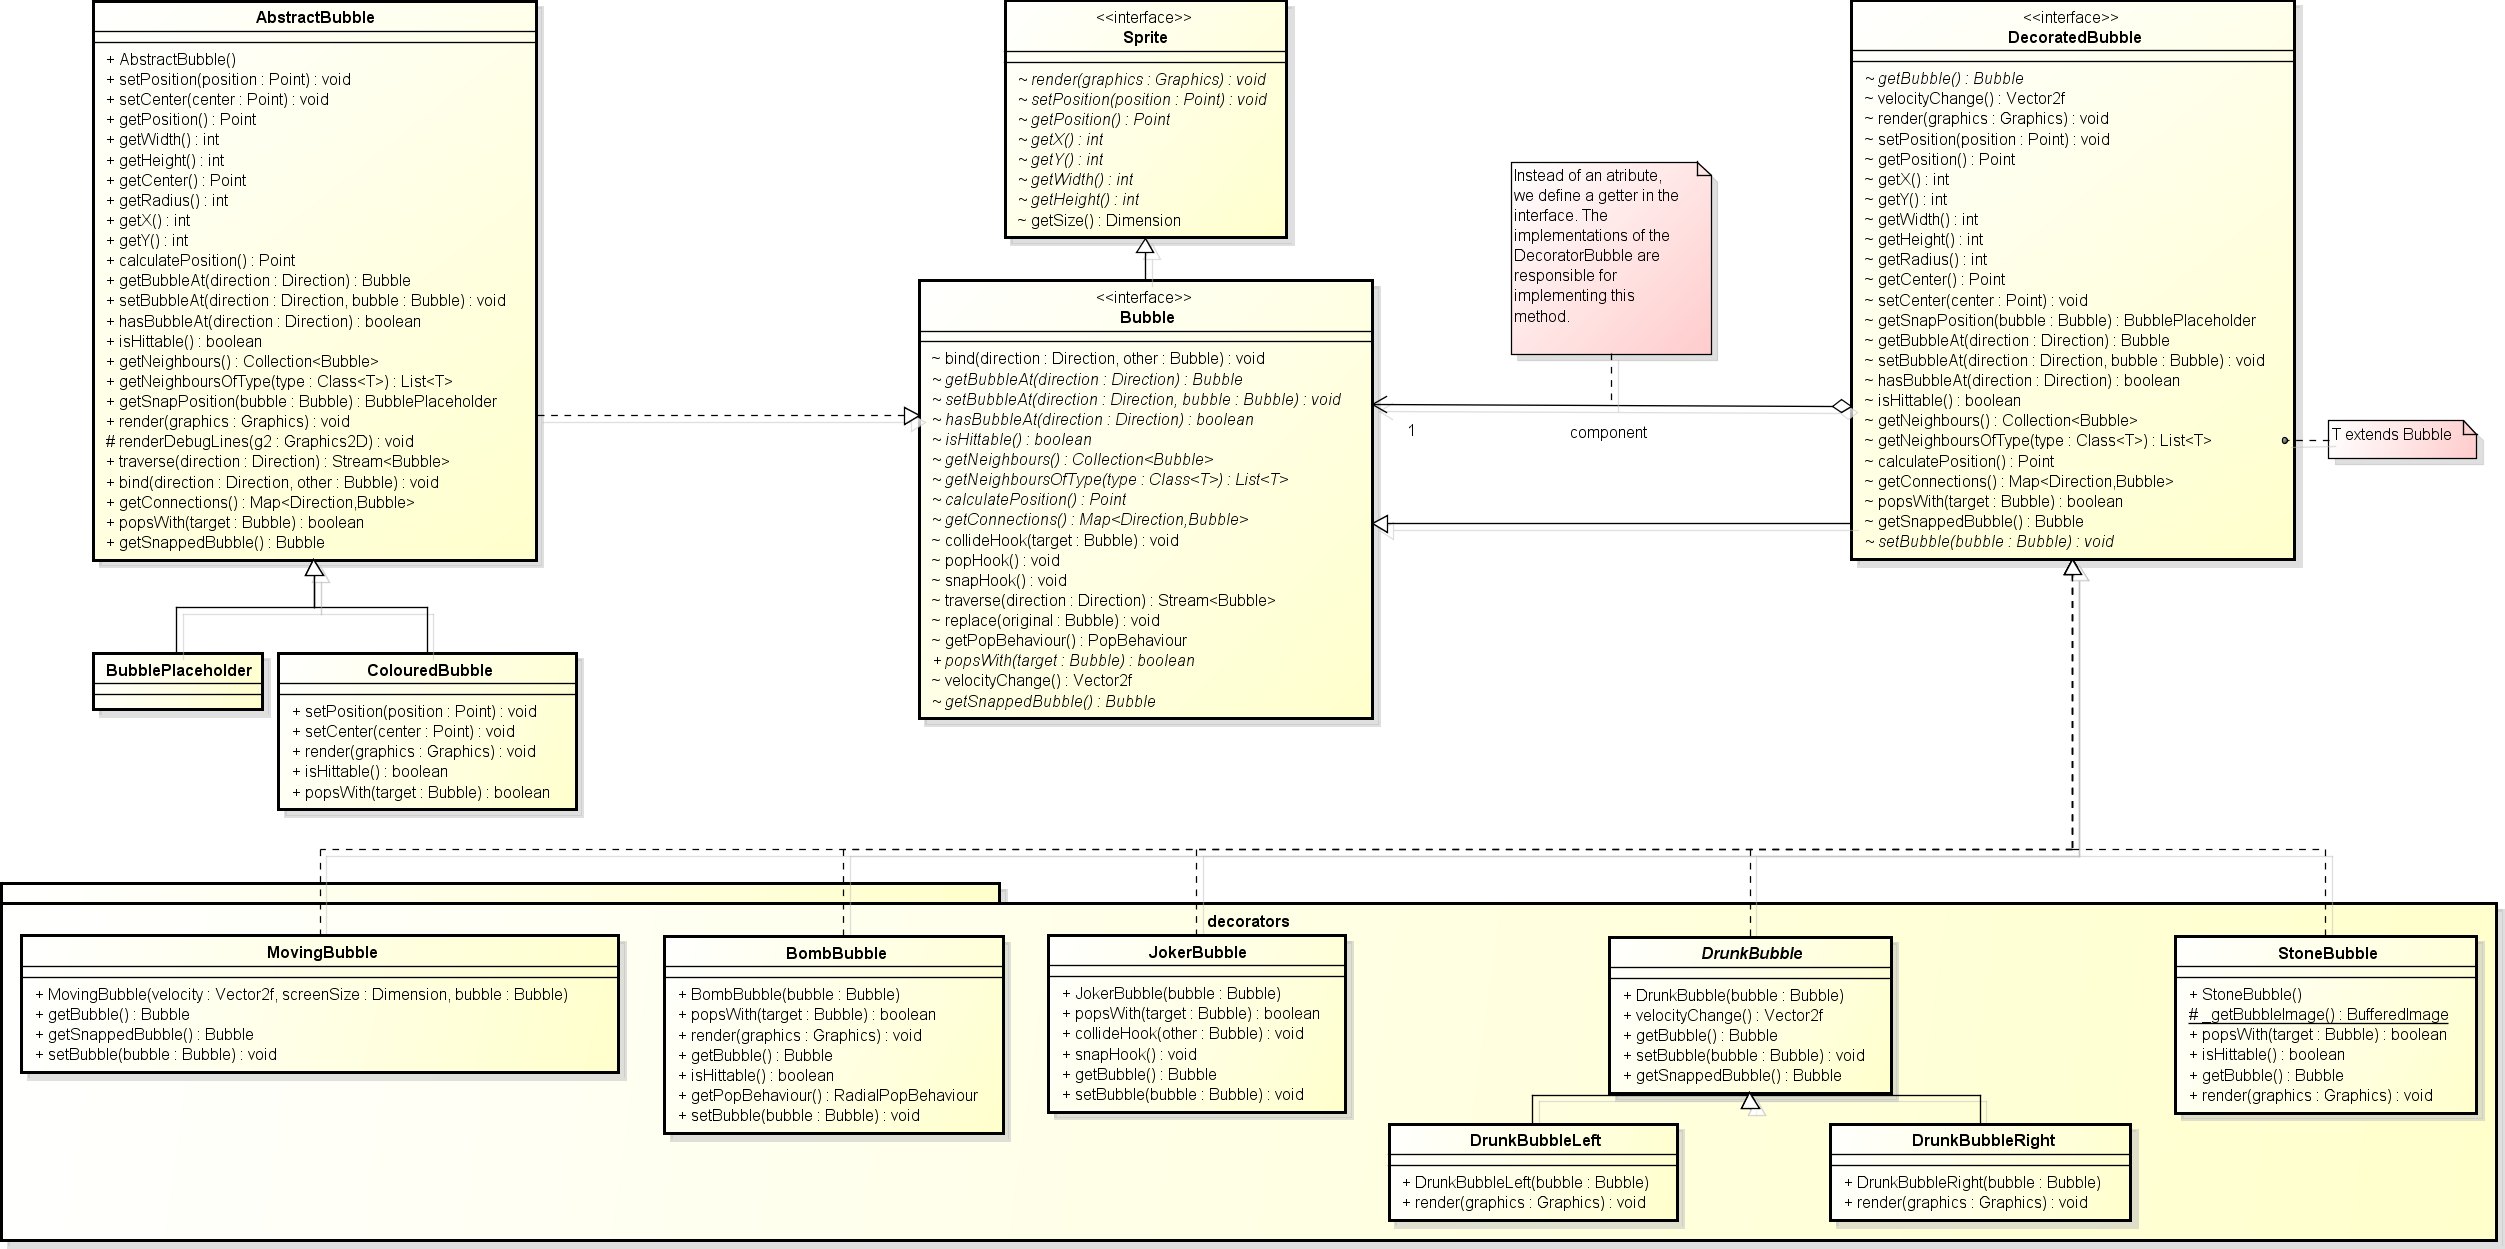
\includegraphics[width=1.0\textwidth]{PowerUpDecoratorClassDiagram.png}
    \caption{\label{fig:PowerUpDecoratorClassDiagram} The class diagram for the implemented decorator pattern}
\end{figure}
\subsubsection{Sequence diagram}
\begin{figure}[H]
    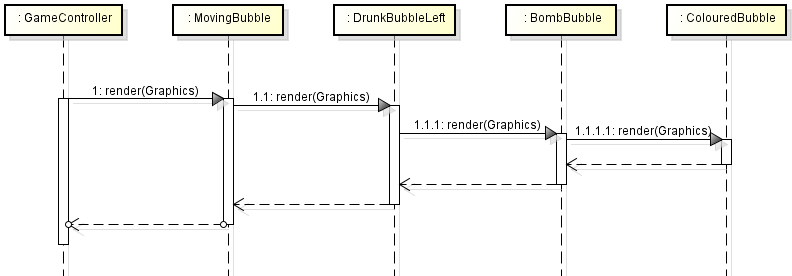
\includegraphics[width=1.0\textwidth]{sequence_decorator_uml_v2.PNG}
    \caption{\label{fig:seq_strategy} A sequence diagram for the implemented decorator pattern}
\end{figure}
All the other methods in the decorator behave in a similar way. Each method will also access the same method in the wrapped object. Some methods will only perform this method call (like MovingBubble and JokerBubble in figure \ref{fig:seq_strategy}), while others will also do more (for example, the render method in DrunkBubbleLeft will also render arrows). This works the same for all combinations of concrete decorators.

\subsection{Strategy}

\subsubsection{Natural language description}
We used the strategy pattern for the pop behaviours of bubbles. Using the strategy pattern makes it possible to add new behaviour without changing other classes. The reason for implementing this pattern was to make the program more flexible, because the behaviours are loosely coupled. This means we can easily add new pop behaviours. This also enables us to give different decorators different pop behaviours.

A PopBehaviour interface was introduced, as displayed in \ref{fig:class_strategy}, which is implemented in the subclasses, each representing a different type of behaviour. For example; the BombBubble pops all nearby bubbles, regardless of their colours. BombBubbles thus have the RadicalPopBehaviour, subclass of PopBehaviour. The normal bubbles, for example, should have different popping behaviour. Here we want to look at the colour of the adjacent bubbles, and we only want to pop them if they are equal in colour and in a group of 3 or more, for which the RecursivePopBehaviour subclass of PopBehaviour is used.

\subsubsection{Class diagram}
\begin{figure}[H]
    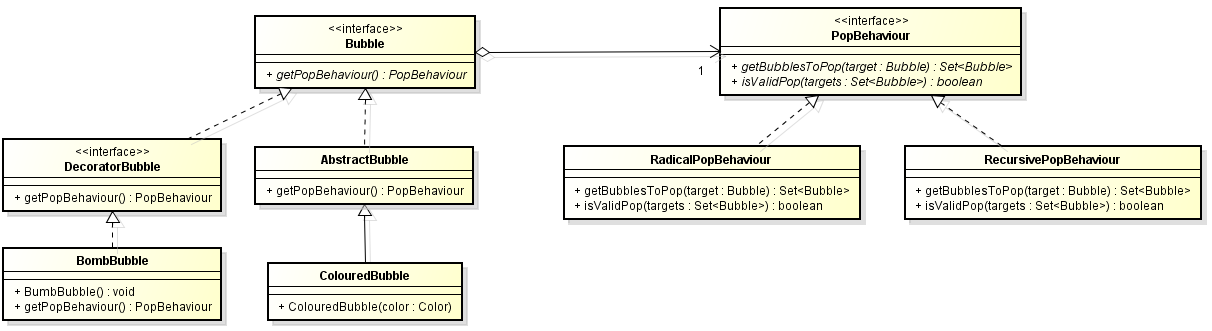
\includegraphics[width=1.0\textwidth]{popping_strategy_class_UML.PNG}
    \caption{\label{fig:class_strategy} The class diagram for the implemented strategy pattern}
\end{figure}

\subsubsection{Sequence diagram}
\begin{figure}[H]
    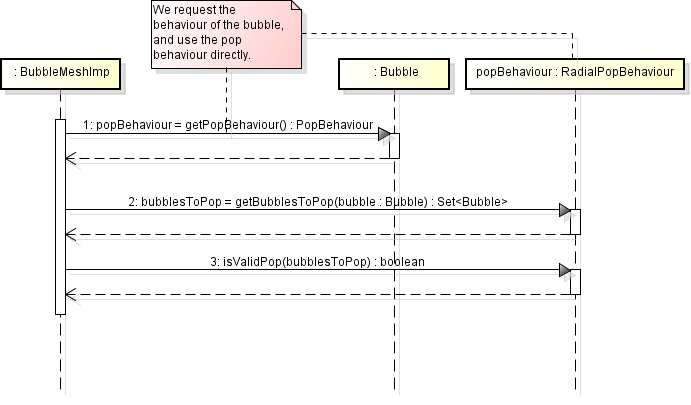
\includegraphics[width=1.0\textwidth]{Seq_RadialPopBehaviour.png}
    \caption{\label{fig:seq_strategy1} The sequence diagram of the RadialPopBehaviour}
\end{figure}
\begin{figure}[H]
    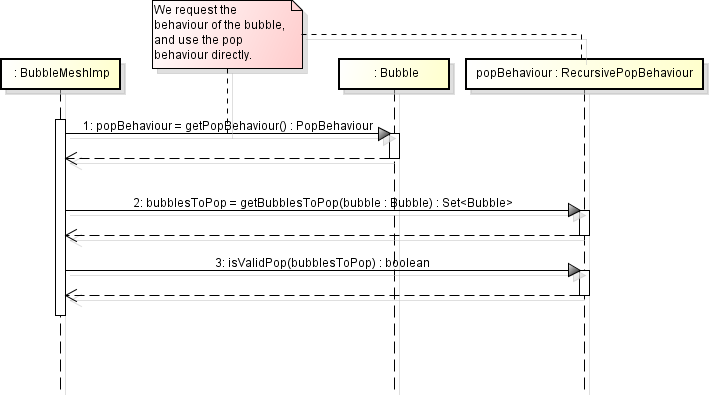
\includegraphics[width=1.0\textwidth]{Seq_RecursivePopBehaviour.png}
    \caption{\label{fig:seq_strategy2} The sequence diagram of the RecursivePopBehaviour}
\end{figure}
For clarification, the return values are named so it is more clear when they are used in successive method calls.

\section{One more design pattern}

\subsection{Model view controller}

\subsubsection{Natural language description}
At the first stages of the development of our game the back-end model logic and GUI logic was heavily intertwined and dependent on each other. We set out to try and get better encapsulation for both through the use of the ModelViewController pattern. However in our implementation there are two MVC's working together. We have a higher level one that controls the game. This higher level one relies on another MVC that handles the Cannon. This does tighten the coupling between the two but in the end they are still quite loosely coupled. The view however doesn't update through observer but it simply requests the models state every cycle. The model however does have an observer and it can notify the higher-level game about changes for multiplayer over the socket.

In the implementation we quickly set up two of both models, controllers and views. The views come together in the GamePanel where they both draw and the listeners are bound between the panel and them. (note: it doesn't appear in the uml because it doesn't affect the structure of the mvc). Because the interfaces needed to be used in two cases they are parameterized interfaces so they could be reused. Furthermore the view $<$C,M$>$ interface binds it all together through the getModel and getController methods (the relationships for the views are actually achieved through this). All in all this gives us a loosely coupled flexible design.


\subsubsection{Class diagram}
\begin{figure}[H]
	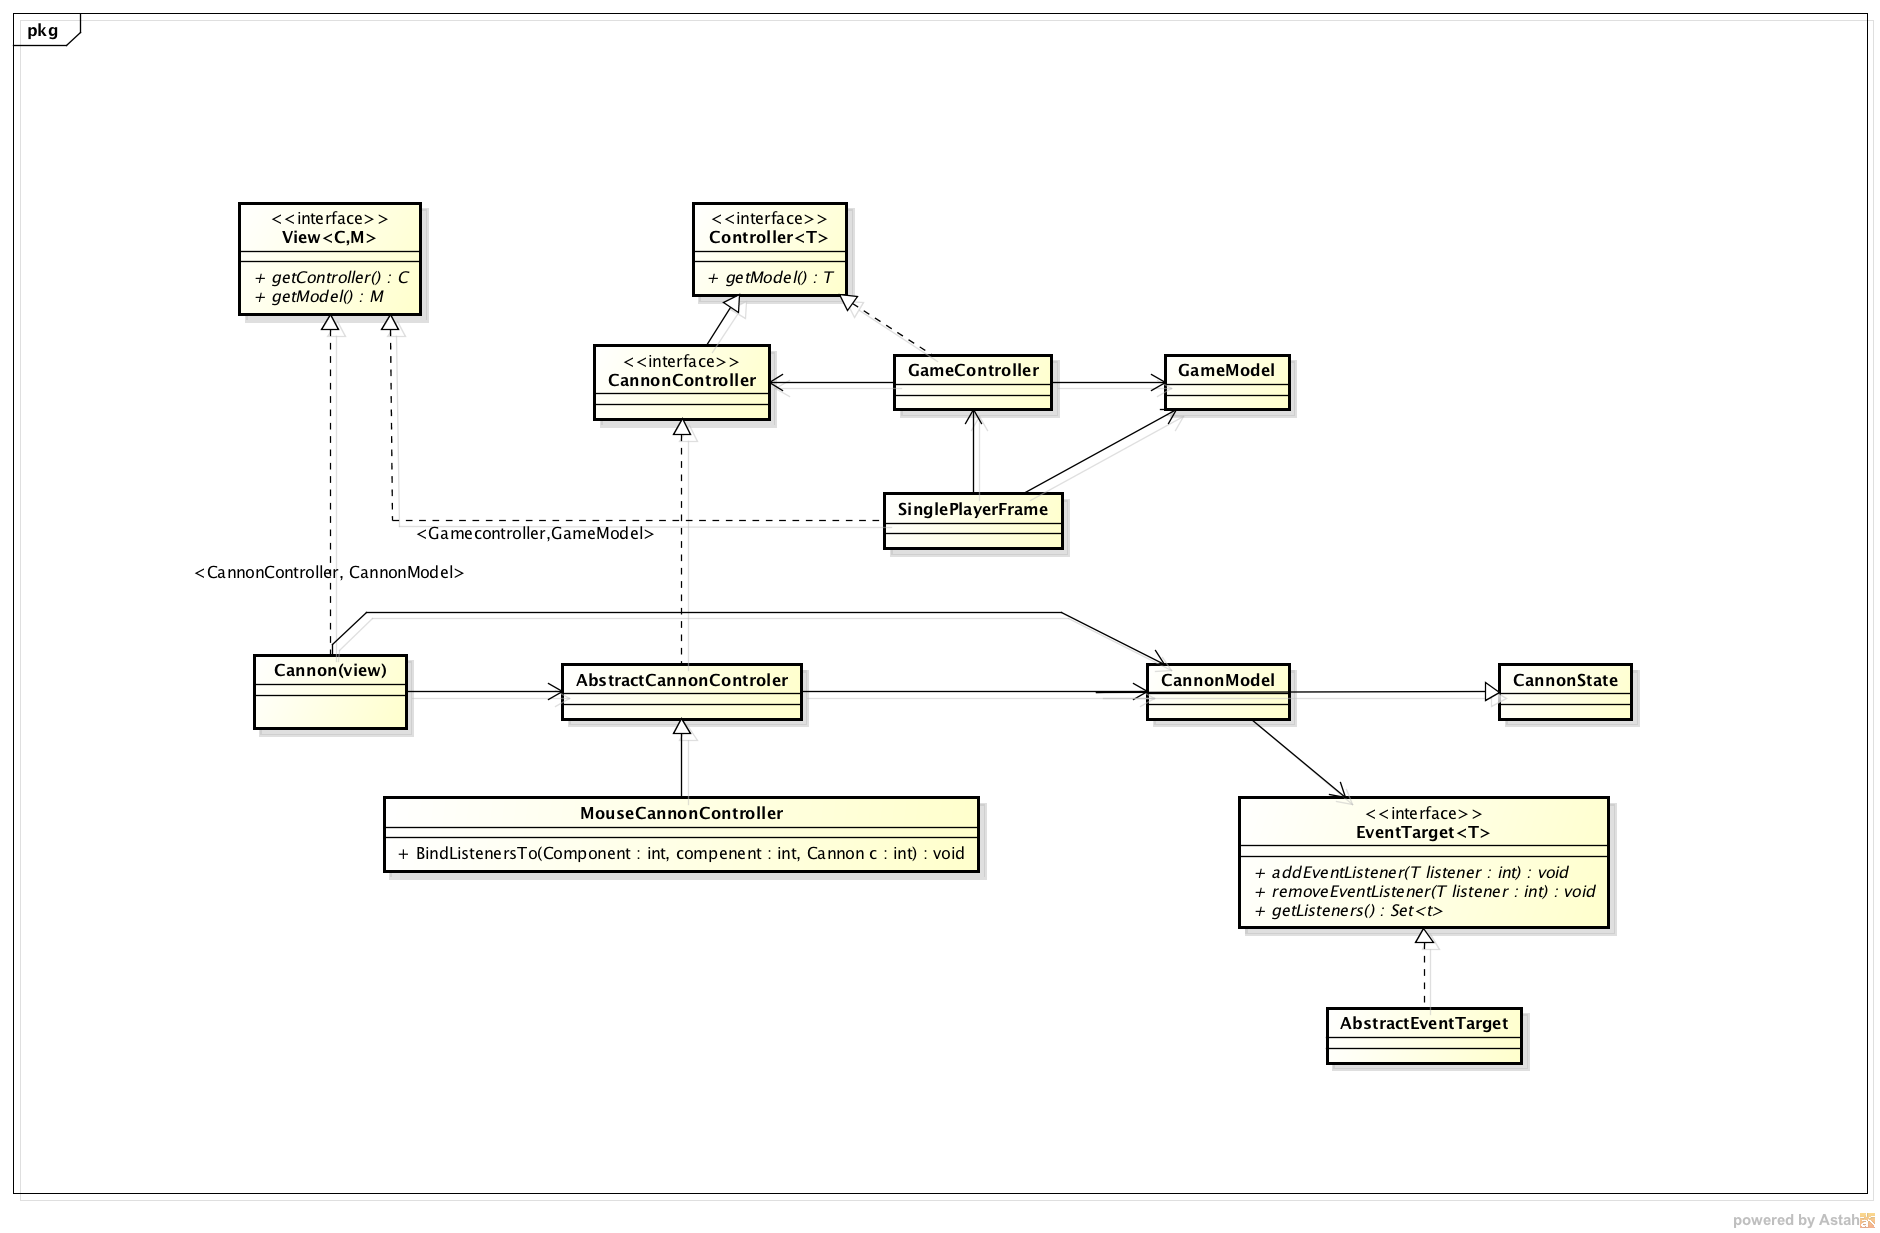
\includegraphics[width=1.0\textwidth]
    {Our_mvc.png}
    \caption{\label{fig:class_mvc}The MVC class diagram}
  \end{figure}

\subsubsection{Sequence diagram}
\begin{figure}[H]
	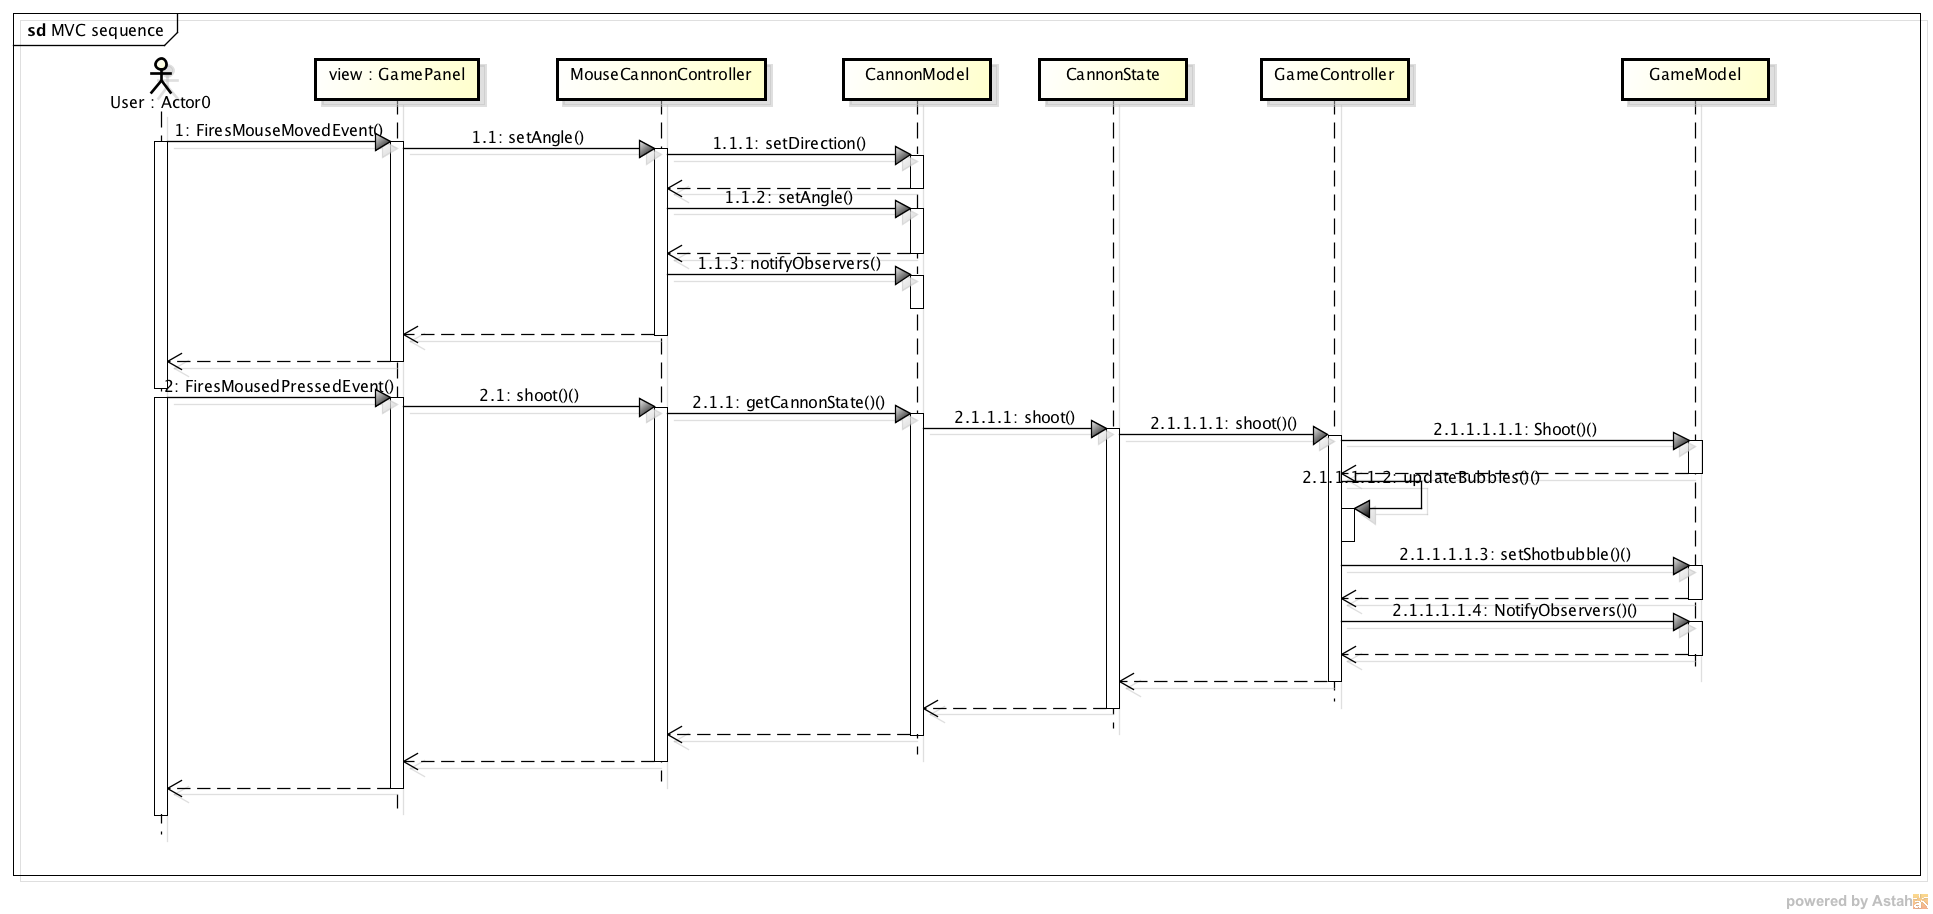
\includegraphics[width=1.0\textwidth]
    {MVC_sequence.png}
    \caption{\label{fig:sequence_mvc}The MVC sequence diagram}
  \end{figure}
  
\end{document}